\documentclass{beamer}

\usetheme[progressbar=foot]{metropolis}           % Use metropolis theme
\metroset{block=fill}

\usepackage{tikz}
\usepackage{url}
\usepackage{amssymb}
\usepackage{amsmath}
\usepackage{amsthm}
\usepackage{appendixnumberbeamer}
\usepackage{xspace}
\usepackage{makecell}
\usepackage{enumerate}
\usepackage[3Dplayspeed=5]{media9}

\newcommand{\code}[1]{\texttt{#1}\xspace}
\newcommand{\pck}{\code{diffpriv}}
\newcommand{\reals}{\ensuremath{\mathbb{R}}\xspace}
\newcommand{\naturals}{\ensuremath{\mathbb{N}}\xspace}
\newcommand{\cB}{\ensuremath{\mathcal{B}}\xspace}
\newcommand{\cD}{\ensuremath{\mathcal{D}}\xspace}
\newcommand{\mech}{\ensuremath{\mathcal{M}}\xspace}
\newcommand{\domain}{\ensuremath{\cD}\xspace}
\newcommand{\eg}{\emph{e.g.},\xspace}
\renewcommand{\Pr}[1]{\ensuremath{\mathrm{Pr}\left(#1\right)}}

\title{Towards Turn-Key Differential Privacy}
\subtitle{Adventures in Function Approximation, \\ Empirical Process Theory and Open-Source Software}
\date{July 25, 2017}
\author{\textbf{Ben Rubinstein}\hfill\textit{joint with Francesco Ald\`a}}
\institute{School of Computing \& Information Systems \hfill
\includegraphics[width=1.5cm]{figures/logo-um} \\ The University of Melbourne}

\begin{document}

\maketitle

\begin{frame}{One More Time With Feeling: Why Protect Privacy?}
\begin{columns}[T,onlytextwidth]
	\column{0.52\textwidth}
	
\includegraphics[width=0.98\columnwidth]{figures/news-netflix} \\[-0.3em]
		\scalebox{0.2}{https://www.wired.com/2010/03/netflix-cancels-contest/}
	\column{0.45\textwidth}
	\hfill
\includegraphics[width=0.98\columnwidth]{figures/news-medicare} \\[-0.5em]
		\hfill\scalebox{0.2}{http://www.abc.net.au/news/2016-09-29/medicare-pbs-dataset-pulled-over-encryption-concerns/7888686}
\end{columns}
\vspace{2em}
Regulatory \& ethical obligations; customer confidence; $\ldots$profits\emph{!!}
\end{frame}

\begin{frame}{DP Successes (If Privacy Doesn't Inspire You)}
\begin{columns}[T,onlytextwidth]
\column{0.4\textwidth}
Recent deployments
\begin{itemize}
\item Google: RAPPOR,\\ Google Chrome
\item Apple: iOS 10.x
\item Uber: SQL Elastic Sensitivity
\item U.S. Census Bureau: OnTheMap
\item Transport for NSW: \\ Opal Data Release
\item etc.
\end{itemize}
\column{0.6\textwidth}
Active world-leading groups: Harvard, Stanford, Berkeley, CMU, Weizmann, UCL, Oxford, USC, UCSD, UPenn, Caltech, Cornell, Duke, Disney Research, Google Research, Microsoft Research, etc. \\

\begin{center}
\includegraphics[width=0.90\columnwidth]{figures/news-godel}\end{center}
\end{columns}
\end{frame}

\begin{frame}{Talk Outline}
\begin{columns}[T,onlytextwidth]
	\column{0.75\textwidth}
	\begin{enumerate}
		\item Intro to differential privacy \\[2.4em]
		\item The Bernstein mechanism: \\ Private function release\\[2.4em]
		\item The sensitivity sampler: \\ Automating privatisation\\[2.4em]
		\item The \pck package
	\end{enumerate}

	\column{0.25\textwidth}
		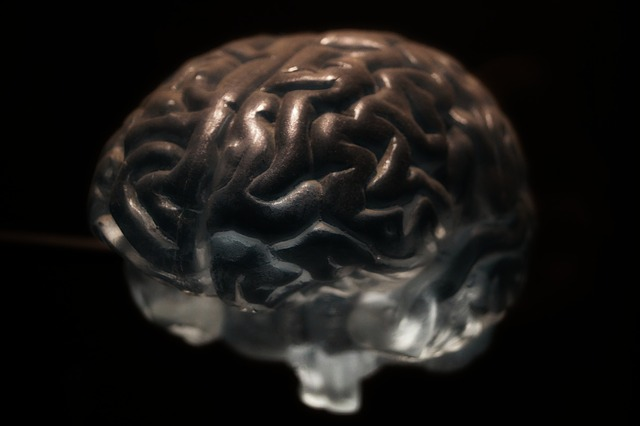
\includegraphics[width=0.98\columnwidth]{figures/brain1}\\
		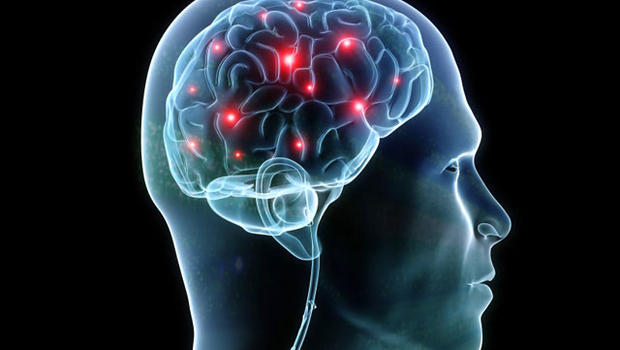
\includegraphics[width=0.98\columnwidth]{figures/brain2}\\
		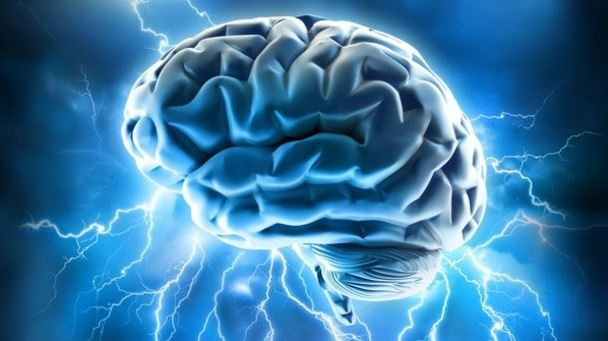
\includegraphics[width=0.98\columnwidth]{figures/brain3}\\
		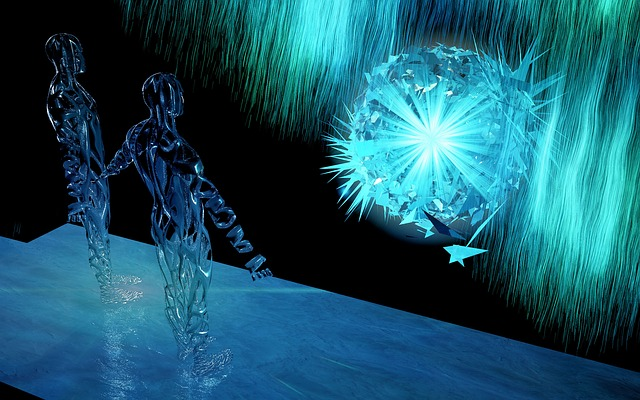
\includegraphics[width=0.98\columnwidth]{figures/brain4}\\[-0.5em]
		\hfill\scalebox{0.4}{CC}
\end{columns}
\end{frame}

\section{Introduction to Differential Privacy}

\begin{frame}{What's DP For?}
	\alert{\emph{Release aggregate information on a dataset, but protect individuals.}} \\[0.5em]
\begin{columns}[T,onlytextwidth]
	\pause
\column{0.9\textwidth}
	%Guarantee meaningful privacy, strive for utility.

	Parties: Trusted data curator; \textbf{Untrusted receipient} \\
	Variations exist \eg decentralised curator \\[0.5em]

	Example \textbf{target analyses} to privatise
\column{0.1\textwidth}
	\hfill
\includegraphics[height=4em]{figures/logo-uscb}
\end{columns}
\begin{itemize}
	\item A function of data: A statistic!
	\item Probabilistic model fitting with MLE: Estimation procedure
	\item Deep neural network training: A learner
	\item KD tree construction: Spatial data analysis
\end{itemize}

\pause In general, privacy/utility must be in tension. \emph{Lower bounds later.}
%Microdata problematic. 
\end{frame}

\begin{frame}{Records, Databases, Target Functions, Mechanisms}
A \alert{database} $D$ is a sequence of $n$ \alert{records} from \alert{domain} set \domain.

A \alert{target function} for privatisation $f: \cD^n \to \cB$ a \alert{response set}

%Typically arbitrary \domain. Arbitrary response space \cB for now.

\begin{exampleblock}{Example: Sample Mean}
Consider releasing the average of scalars, \eg test scores \\
\domain=\cB=\reals and $f(D)=\frac{1}{n}\sum_{i=1}^n D_i$
\end{exampleblock}

\texttt{> D <- rnorm(1000) \textit{\# 1000 standard normal samples}}\\
\texttt{> f <- mean}\\
\texttt{> f(D)} \\
\texttt{[1] 0.03339015}

\end{frame}

\begin{frame}{Records, Databases, Target Functions, Mechanisms (cont.)}
A \alert{mechanism} $\mech$ maps $D$ to a \alert{random response} in \cB. \\
\alert{Response distribution}: $\Pr{\mech(D)\in B}$ for $B\subset\cB$. 

\begin{center}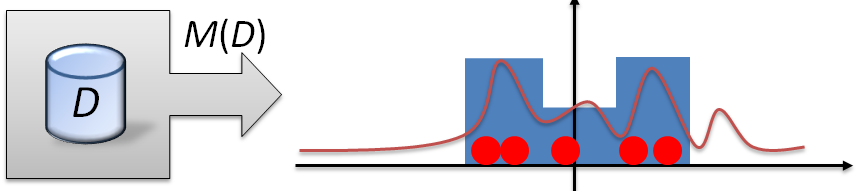
\includegraphics[width=0.8\textwidth]{figures/mechanism}\end{center}

\pause
\begin{exampleblock}{Example: Blood Type}
Everyone in $D$ have same blood type?  $f(D) = 1[D_1=\ldots=D_n]$. \\
\begin{columns}[T,onlytextwidth]
\column{0.4\textwidth}
\vspace{1.3em}
$\mech(D)\sim Bernoulli(0.5)$
\column{0.6\textwidth}
$\mech(D) = \begin{cases} f(D)\ , & w.p.\ 0.9\ , \\ 1 - f(D) & w.p.\ 0.1 \end{cases}$
\end{columns}
\end{exampleblock}

\alert{Utility} measures (high probability) proximity of $\mech(D), f(D)$


\end{frame}

\begin{frame}{Defining Differential Privacy}
%When probabilities are non-zero: $\log\left(\frac{\Pr{\mech(D)\in B}}{\Pr{\mech(D')\in B}}\right)\leq\epsilon$
Intuition: Response indistinguishable on changing any one record
\begin{center}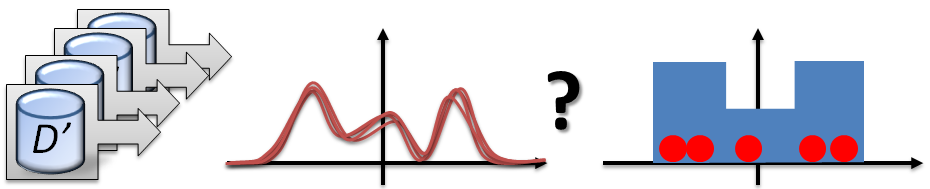
\includegraphics[width=0.8\textwidth]{figures/indistinguishable}\end{center}

Databases $D, D'$ are called \alert{neighbouring} if they differ on one record

\pause
\begin{alertblock}{\mech is $\epsilon$-Differentially Private}
If for all neighbouring $D, D'\in\domain^n$, for all $B\subset\cB$, we have that 
$\Pr{\mech(D)\in B}\leq\exp(\epsilon)\cdot\Pr{\mech(D')\in B}$. Where $\epsilon>0$.
\end{alertblock}

That is $\log\left(\frac{\Pr{\mech(D)\in B}}{\Pr{\mech(D')\in B}}\right)\leq\epsilon$:
Smaller $\epsilon>0$, more privacy.

Semantic privacy with strong threat model; \emph{worst-case on DBs.}
\end{frame}

\begin{frame}{Example: Numeric Releases with the Laplace Mechanism}
Consider target $f: \domain \to \reals^d$ \\
\textit{\eg a covariance matrix, regression coefficients, classifier weights}

Smooth the target by adding zero-mean Laplace noise to output.

\begin{alertblock}{Laplace Mechanism}
Given parameters $\Delta, \epsilon>0$, release 
$\mech(D) \sim f(D) + Lap(\Delta / \epsilon)$.
\end{alertblock}

\begin{center}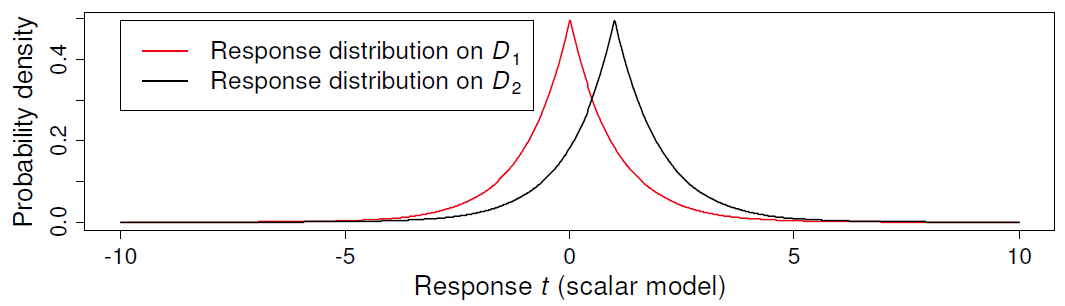
\includegraphics[width=1.0\textwidth]{figures/laplace-proof}\end{center}

\end{frame}

\begin{frame}{Example: Hello World -- Sample Mean of $D_i\in [0,1]$}
	\includemedia[label=laplace, activate=pageopen, width=1\textwidth, height=0.64122\textwidth, addresource=laplace.mp4, flashvars={source=laplace.mp4}]{}{VPlayer.swf}
\end{frame}

\begin{frame}{Global Sensitivity}
Many generic mechanisms like Laplace operate by smoothing $f$. \\
Less smoothing needed for already-smooth $f$; How to measure? \\[1em]

Consider target $f: \domain \to \cB$ with \alert{normed response space} \cB.

\pause
\begin{alertblock}{Global sensitivity}
$\Delta(f) = \max_{D,D'} \|f(D) - f(D')\|_\cB$ over neighbouring DBs in $\domain^n$.
\end{alertblock}
A type of Lipschitz condition. (Weakest form of smoothness.)

\begin{exampleblock}{Example: Sample Mean}
Take $f(D)=\frac{1}{n}\sum_{i=1}^n D_i$ in $\cB=\mathbb{R}$, with absolute as norm. \\
If $D_i\in[0,1]$ then $\Delta(f)= 1/n$.
\end{exampleblock}
\end{frame}

\begin{frame}{Privacy of the Laplace Mechanism}

Recall
\begin{itemize}
\item $\Delta(f) = \max_{D,D'} \|f(D) - f(D')\|_\cB$ over neighbouring DBs.
\item $\mech(D) \sim f(D) + Lap(\Delta / \epsilon)$.	
\end{itemize}
\begin{alertblock}{Theorem: Laplace Mechanism Privacy}
	If $\Delta$ is $L_1$-gobal sensitivity of $f$, then $\mech$ is \alert{$\epsilon$-DP.} %Note $\|x\|_1=\sum_i |x_i|$.
\end{alertblock}
\textbf{Why $L_1$?} \textit{multivariate Laplace has density exponential in $L_1$.} \\[1.0em]

\pause
More privacy (smaller $\epsilon$), the more noise needed, lower utility. \\
The smoother the target (low $\Delta)$, the less smoothing needed.

%\emph{Proof.} For any $t\in\reals$, neighbouring $D,D'$
%\begin{eqnarray*}
%	\frac{p(\mech(D)=t)}{p(\mech(D')=t)} &=& \frac{\exp(-\|f(D) - t\|_1 \cdot \epsilon / \Delta)}{\exp(-\|f(D')-t\|_1 \cdot \epsilon / \Delta } \\
%	&=& \exp\left( - (\|f(D)-t\|_1 - \|f(D') - t\|_1) \cdot \epsilon / \Delta\right) \\
%	&\leq& \exp(\|f(D)-f(D')\|_1 \cdot \epsilon / \Delta) 
%	\leq \exp(\epsilon) \enspace. \hfill\qed
%\end{eqnarray*}
\end{frame}

\begin{frame}{Notes}
	\begin{itemize}
		\item \alert{Generic mechanisms} like Laplace have driven DP's ascent
		\item Another driver: A calculus of \alert{composition}
		\item Many applications explored in telecom, health, web, etc.
		\item \alert{Utility bounds} exist for simpler mechanisms: Guide choices
		\item Empirical investigations: some mechanisms work, some don't
		\item \alert{Lower bounds} illustrate impossibility results
	\end{itemize}
\end{frame}

\section{The Bernstein Mechanism: \\ Private Function Release -- AAAI'17}

\begin{frame}{Bernstein vs. Laplace Mechanisms}
\textbf{Problem:} What about \alert{releasing a function}? A trained classifier? \\

\begin{center}\scalebox{0.8}{
	\begin{tabular}{lcc}
		\Xhline{3\arrayrulewidth}
		& \textbf{Laplace Mechanism}	& \textbf{Bernstein Mechanism} \\
		\Xhline{3\arrayrulewidth}
		\textit{Operation} \\
		\;\;\;\;Response space \cB	& $\reals^d$		& functions: $[0,1]^d\to\reals$ \\
		\;\;\;\;Perturbation		& output		& output \\
		\hline
		\textit{Privacy} \\
		\;\;\;\;Requires access to		& $f(D)$, $\Delta(f)$	& $f(D)$, $\Delta(f)$ \\
		\;\;\;\;Sensitivity norm	& $L_1$			& $L_1$ of $f(\cdot)$ evaluated on lattice \\
		\;\;\;\;Privacy guarantee	& $\epsilon$-DP		& $\epsilon$-DP \\
		\hline
		\textit{Utility} \\
		\;\;\;\;Conditions		& -			& Smooth $f(\cdot)$ \\
		\Xhline{3\arrayrulewidth}
	\end{tabular}
}\end{center}
\end{frame}

\begin{frame}{Bernstein Mechanism: Sketch}
\textbf{Goal}: Privately release function $g$ returned by $f: \domain^n \to \reals^{[0,1]^d}$ \\
\textbf{Parameters}: degree $k$, sensitivity $\Delta$, privacy $\epsilon>0$ \\

\begin{enumerate}
	\pause \item Function $g \longleftarrow$ \alert{Evaluate} $f(D)$
	\pause \item Coefficients $\mathbf{c} \longleftarrow$ \alert{Approximate} $g$ on a grid over $[0,1]^d$
	\pause \item Coefficients $\tilde{\mathbf{c}} \longleftarrow$ \alert{perturb} $\mathbf{c}$ by Laplace mechanism
	\pause \item \alert{Release} coefficients $\tilde{\mathbf{c}}$
\end{enumerate}
\pause \alert{Reconstruct} release function
\begin{enumerate}
	\item[4.] $\tilde{g} \longleftarrow$ perturbed coefficients $\tilde{\mathbf{c}}$, dot, public basis functions
\end{enumerate}
\end{frame}

\begin{frame}{Aside: Bernstein Function Approximation}
\textbf{Goal}: Approximate $g: [0,1]\to\reals$ by smooth polynomial

\pause Degree-$k$ \alert{basis} $b_{\nu,k}(x)={k\choose\nu}x^\nu(1-x)^{k-\nu}$ for $\nu\in\{0,\ldots,k\}$

\pause \alert{Coefficients} $\mathbf{c}$: evaluations on \alert{grid} $g(0/k), g(1/k), \ldots, g(k/k)$

\pause \alert{Bernstein operator}: $g(x)\approx \sum_{\nu=0}^k g(\nu/k) b_{\nu,k}(x)$

\begin{center}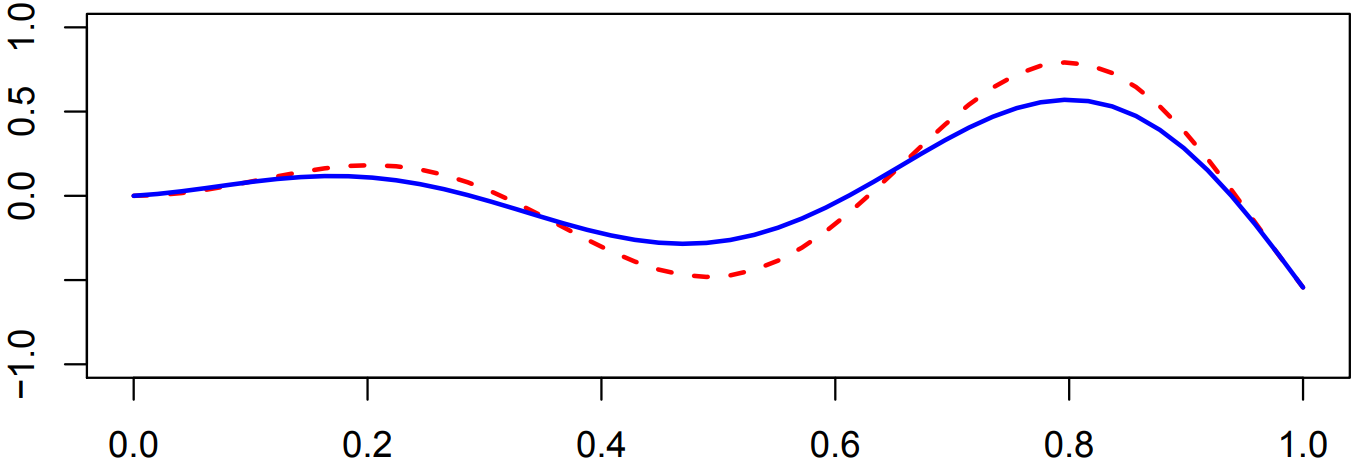
\includegraphics[width=0.8\textwidth]{figures/results-bernstein-poly}\\ $k=50$\end{center}
\end{frame}

\begin{frame}{Bernstein Utility}
	\begin{columns}[T,onlytextwidth]
		\column{0.55\textwidth}
			\begin{alertblock}{Utility: $\leq\alpha$ error whp $\geq 1-\beta$}
			\begin{enumerate}
				\item $(2h,T)$-smooth target: $\alpha=O\left(\frac{\Delta}{\epsilon}\log\frac{1}{\beta}\right)^{\frac{h}{d+h}}$ \\
				\item $(\gamma,L)$-H\"older continuous: $\alpha=O\left(\frac{\Delta}{\epsilon}\log\frac{1}{\beta}\right)^{\frac{\gamma}{2d+\gamma}}$ \\
				\item Linear target: $\alpha=O\left(\frac{\Delta}{\epsilon}\log\frac{1}{\beta}\right)$
			\end{enumerate}
			\end{alertblock}
		\column{0.45\textwidth}
			\vspace{1em}
			\hfill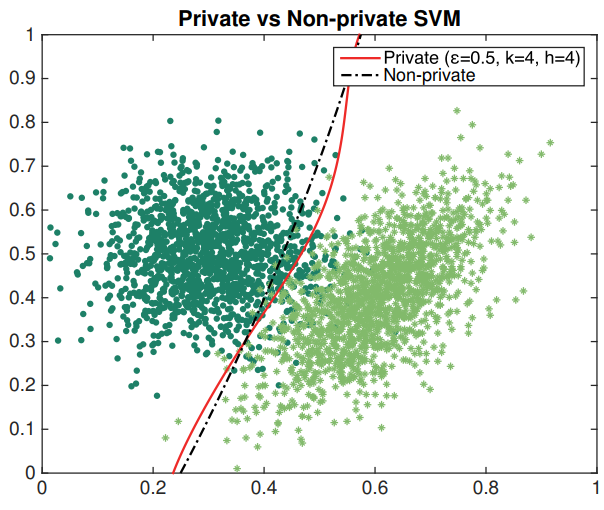
\includegraphics[width=0.95\textwidth]{figures/results-bernstein-svm}
	\end{columns}

	\pause Proschan'65: Concentration of convex comb of iid log-concave rv \\
	Weierstrass Theorem: uniform approximation \\[0.5em]

	\pause \alert{Lower bound}: There exists a target s.t. all $\epsilon$-DP mechanisms introduce $\geq\Omega(\Delta/\epsilon)$ error with probability going to $1$
\end{frame}

\section{The Sensitivity Sampler: \\ Automating Privatisation -- ICML'17}

\begin{frame}{\alert{``Just bound sensitivity''} he said, ``It will be great'' he said.}
	%Generic mechanisms (Laplace, Bernstein) are great, 
%\alert{``Just bound global sensitivity}'' he said, ``It will be great'' he said.\\
\pause Bound sensitivity for releasing SVM classifier (Rubinstein et al. 12)
\begin{center}
%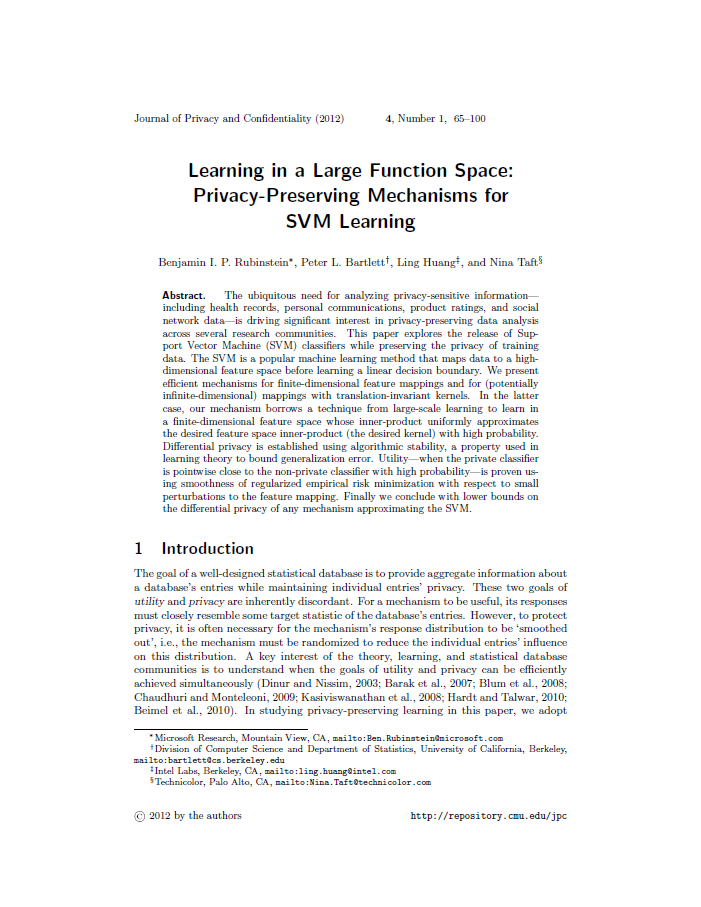
\includegraphics[width=0.3\textwidth]{figures/paper-svm-1}
%\hfill
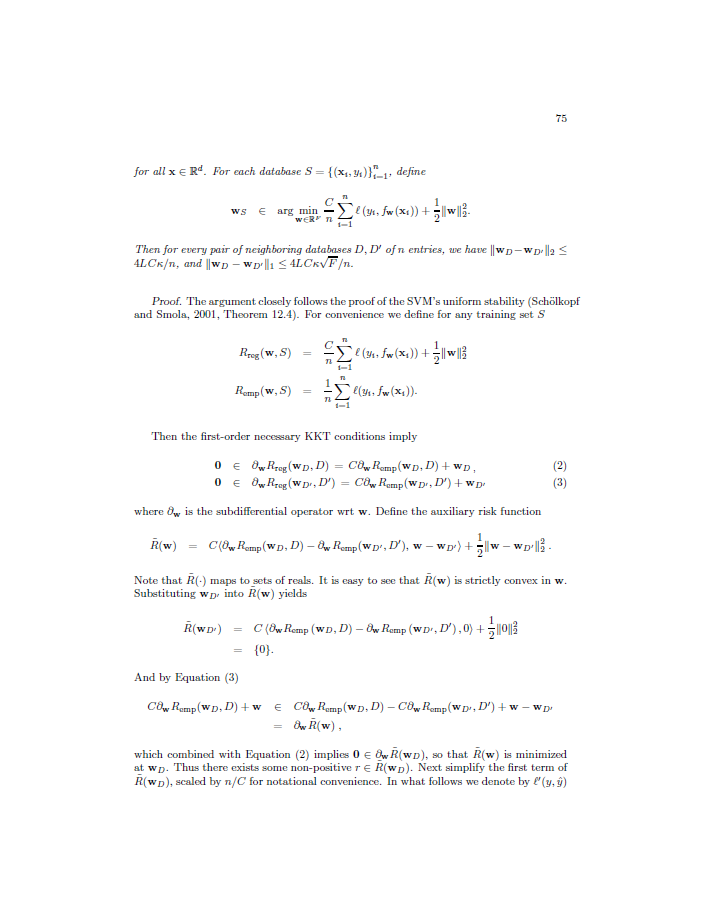
\includegraphics[width=0.49\textwidth, trim={0cm 3.5cm 0cm 3.5cm}, clip]{figures/paper-svm-2}
\hfill
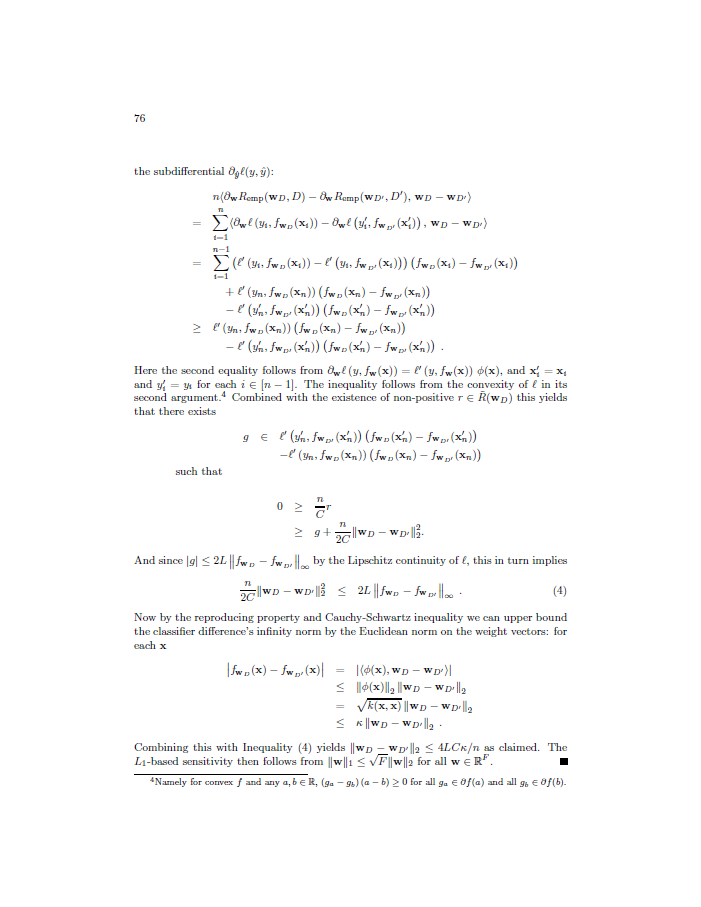
\includegraphics[width=0.49\textwidth, trim={0cm 3.5cm 0cm 3.5cm}, clip]{figures/paper-svm-3}
\end{center}
\pause Simple? Subdifferentials, algorithmic stability, convex auxiliary risk 
\end{frame}

\begin{frame}{``Laws of Mathematics are Very Commendable but...''}
\pause
Apply generic mechanisms without bounding sensitivity?\\[1em]

\textbf{Existing work}: \alert{Restrict targets} until sensitivity can be `composed' \eg recent Uber/Berkeley Elastic Sensitivity system. \\[1em]

\textbf{This work}: Permit \emph{any} target, but won't bound target sensitivity over all DB pairs. Instead \alert{sensitivity over all reasonable DBs}. \\[1.0em]

Key ideas
\begin{itemize}
	\item High-prob bound on sensitivity $\Rightarrow$ Mechanisms \alert{probably DP}
	\item \alert{Sampling}, \alert{Emp process theory} $\Rightarrow$ High-prob sensitivity bound 
\end{itemize}
\end{frame}

\begin{frame}{Idea 1: Sensitivity-Induced Privacy}
%Let's unpack the role of target sensitivity on mechanism DP.
\begin{block}{Mechanism $\mech$ (on target $f$) is \alert{sensitivity-induced private}}
If for neighbouring $D,D'$: $\|f(D)-f(D')\|_\cB\leq\Delta$ implies $\forall B\subset\cB, \Pr{\mech_\Delta(D)\in B}\leq\exp(\epsilon)\cdot\Pr{\mech_\Delta(D')\in B}$
\end{block}

%\begin{exampleblock}{Sensitivity-induced private mechanisms?}
%Most! Laplace, Gaussian, exponential, Bernstein and more.
%\end{exampleblock}

\alert{Many mechanisms!} Laplace, Gaussian, exponential, Bernstein\\[0.5em]

Connecting the dots:
\begin{itemize}
\item Choose a `natural` distribution $P$ on \cD
\item $\Pr{\mbox{$\mech_\Delta$ being $\epsilon$-DP on $D,D'$}} \geq \Pr{\|f(D)-f(D')\|_\cB\leq\Delta}$
\item \alert{$(\gamma,\epsilon)$-random DP} (Hall et al. 2012): \\
$\Pr{\mbox{$\mech_\Delta$ being $\epsilon$-DP on $D,D'$}} \geq 1 - \gamma$ \\
Intuition: DP on most databases, ignore the pathological.
\end{itemize}

%Higher $\Delta$: Lower utility, Higher RDP confidence, but how much?

%DP demands close response distributions over all DB pairs. \\

%These mechanisms being DP follows from $\Delta$ worst-case sensitivity %\\[1em]

%%Let's aim for response distribution closeness on `likely' DB pairs. 
\end{frame}

\begin{frame}{Idea 2: Sample and Estimate $\Pr{\|f(D)-f(D')\|_\cB\leq\Delta}$}
Define $G=\|f(D)-f(D')\|_\cB$ from neighbouring $D,D'\sim P^n$
\begin{itemize}
\item \alert{CDF of $G$} is $\Pr{\|f(D)-f(D')\|_\cB\leq\Delta}$
\item Idea 1: $\mech_\Delta$ is RDP with confidence $1-\gamma=CDF(\Delta)$
\item \alert{Compute then invert} $\Delta=CDF^{-1}(1-\gamma)$? ...\emph{groan}
\end{itemize}
\vspace{-0.5em}
\pause
\begin{columns}[T,onlytextwidth]
\column{0.60\textwidth}
\begin{block}{Algorithm: \alert{Sensitivity-sampler}}
\begin{enumerate}
	\item Sample target: $G_1,\ldots,G_m\sim G$
	\item Empirical CDF: $\frac{1}{m}\sum_{i=1}^m 1[G_i\leq\Delta]$
	\item Dvoretsky-Kiefer-Wolfowitz: \\ ECDF $\rho'$ close to CDF, whp $1-\rho$
	\item $\Delta=ECDF^{-1}(1-\gamma+\rho+\rho')$
\end{enumerate}
\end{block}
\column{0.40\textwidth}
\vspace{1.5em}
\hfill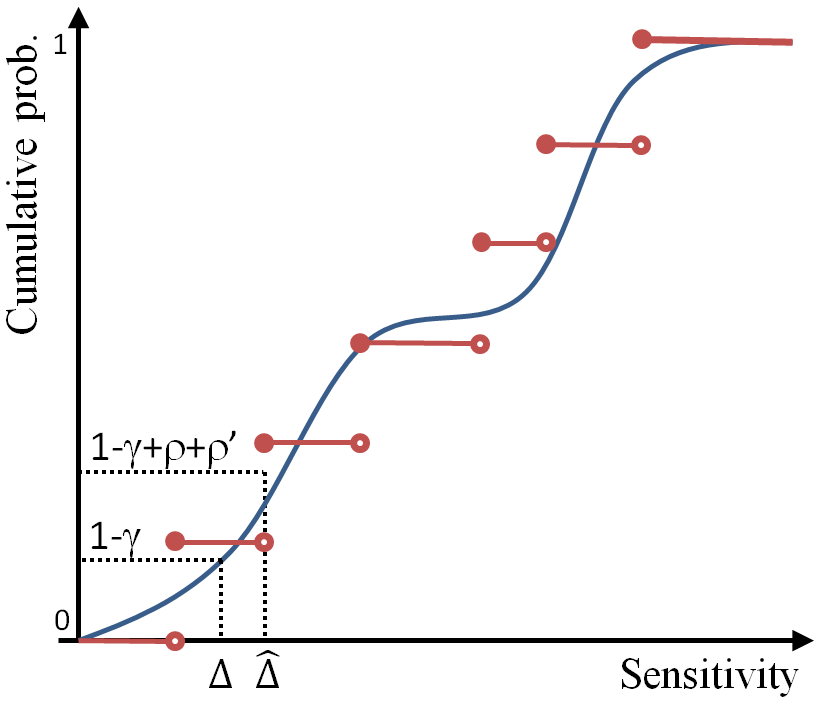
\includegraphics[width=0.98\columnwidth]{figures/samplerhowto}
\end{columns}
\end{frame}

\begin{frame}{Example: Priestly-Chao Kernel Regression}
\includemedia[label=sampler, activate=pageopen, width=1\textwidth, height=0.57191\textwidth, addresource=sampler.mp4, flashvars={source=sampler.mp4}]{}{VPlayer.swf}
\end{frame}

\begin{frame}{Density Estimation: Utility vs Privacy}
	\vspace{1em}
	\begin{center}
		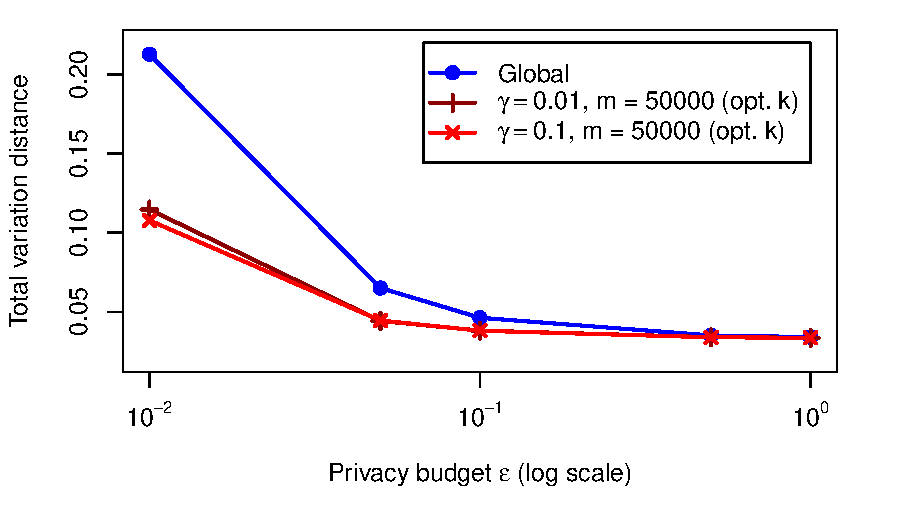
\includegraphics[width=1\textwidth]{figures/KDE_utility_vs_privacy}
	\end{center}
	\vspace{-1em}
	Synthetic $n=5000$ (1000 repeats); Bernstein with $k=10, h=3$%; Asymptote due to Bernstein approx error
\end{frame}

\begin{frame}{Notes}
When resource constrained, can strike \alert{`optimal' trade-offs}: \\
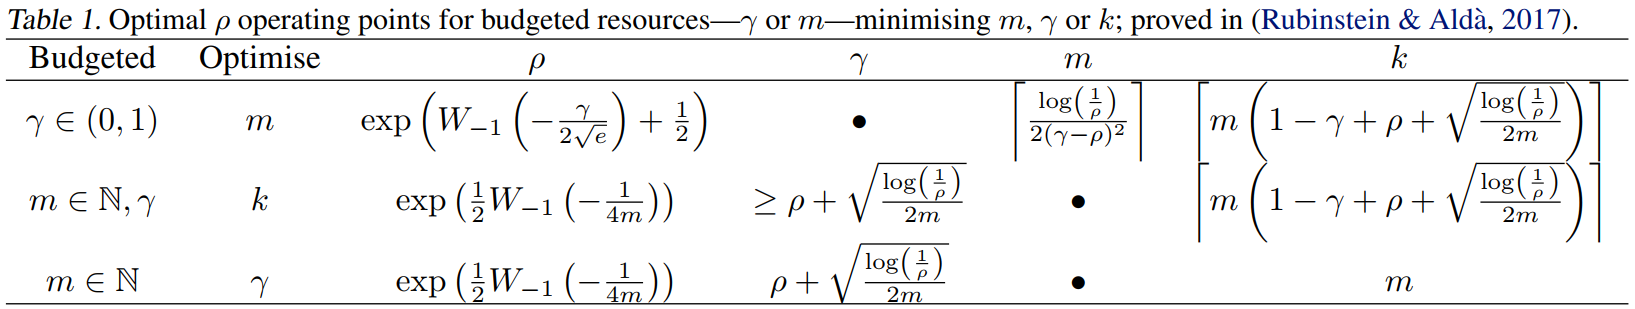
\includegraphics[width=1.0\textwidth]{figures/oppts} \\[0.8em]
\begin{columns}[T,onlytextwidth]
\column{0.7\textwidth}
Estimate \alert{sensitivity offline \& in parallel}
\begin{itemize}
\item $m$ up, then RDP confidence $1-\gamma$ up
\end{itemize}
\vspace{0.5em}
\alert{Distribution $P$} on records:
\begin{itemize}
	\item Non-informative \eg uniform, Gaussian
	\item A (public) Bayesian prior
	\item Density fit privately to data
\end{itemize}
\column{0.3\textwidth}
\vspace{0.5em}
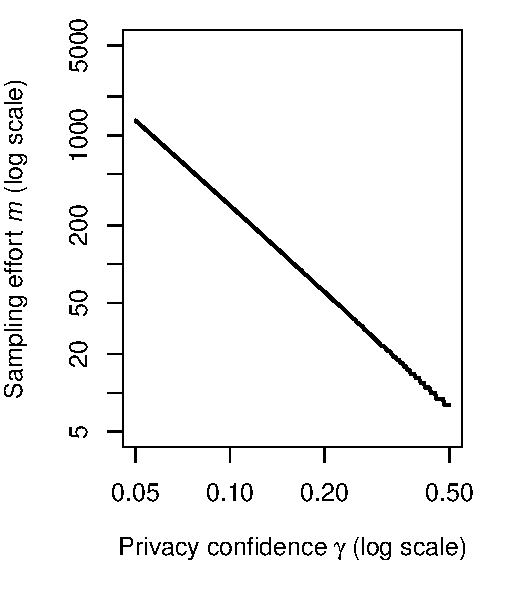
\includegraphics[width=1\columnwidth]{figures/m-vs-gamma}
\end{columns}
\end{frame}

\section{The \pck Package}

\begin{frame}{\pck on CRAN and GitHub \hfill \alert{Google: `diffpriv R'}}

\newcommand{\lb}{\linebreak[4]\vspace{-0.2em}}

	\begin{columns}[T,onlytextwidth]
		\column{0.7\textwidth}
			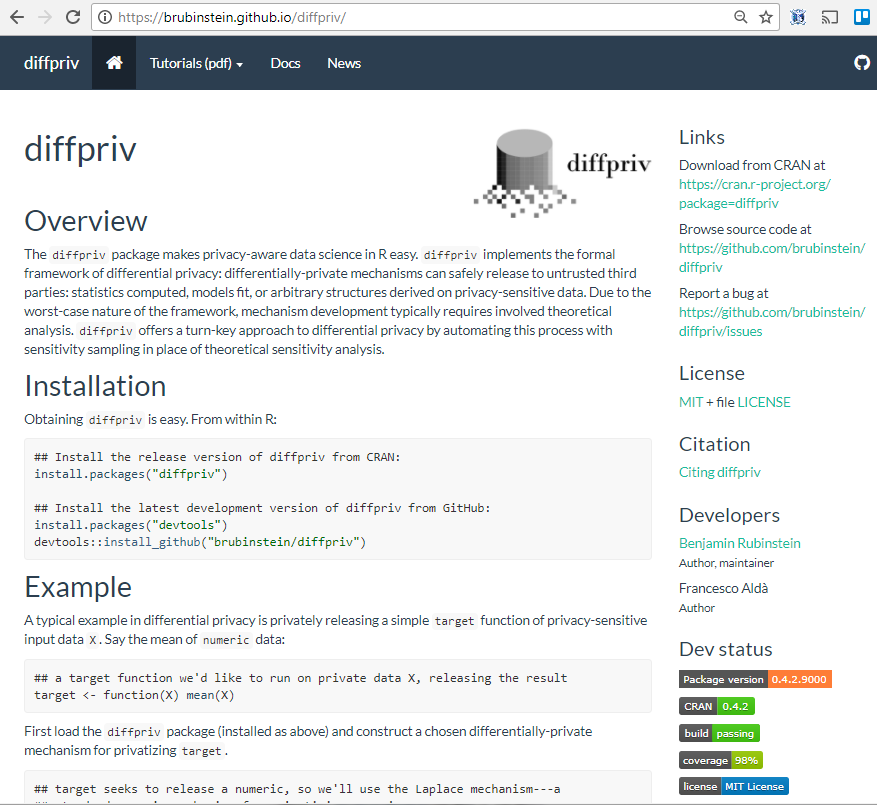
\includegraphics[width=0.95\columnwidth]{figures/screenshot-homepage}
		\column{0.3\textwidth}
			Open-source R  \lb

			`Official' on CRAN with rigorous submission process \lb

			\code{roxygen2} docs \lb

			Tutorial vignettes \lb

			98\% Codecov \lb

			Travis CI
	\end{columns}

\end{frame}

\begin{frame}[standout]
\code{install.packages("diffpriv")}
\end{frame}

\begin{frame}{Architecture Highlights\hfill
\includegraphics[height=1.2em]{figures/logo-diffpriv-alert}}

\code{DPMech}: \code{VIRTUAL S4} class for sensitivity-induced mechanisms
\begin{enumerate}
	\item Slot \code{target}: The non-private target function $f$
	\item Slot \code{sensitivity}: Sensitivity of $f$ to calibrate mechanism \label{dpmech:sensitivity}
	\item \code{releaseResponse()}: Sample from response distribution
	\item \code{sensitivityNorm()}: $\Delta_f(D_1,D_2)=\|f(D_1)-f(D_2)\|_{\cB}$ \label{dpmech:norm}
	\item \code{sensitivitySampler()}: Probes \#\ref{dpmech:norm} to fill \#\ref{dpmech:sensitivity}
\end{enumerate}

\pause
Included generic mechanisms, all subclass \code{DPMech}
\begin{itemize}
	\item \code{DPMechLaplace}, \code{DPMechGaussian}: numeric release
	\item \code{DPMechExponential}: private optimisation
	\item \code{DPMechBernstein}: function release
\end{itemize}
\end{frame}

\begin{frame}{Conclusions}

\newcommand{\lb}{\linebreak[4]\vspace{-0.2em}}

Differential privacy 
\begin{itemize}
	\item Semantic privacy; practical in many ways; complements cryto
	\item Many deep connections between TCS, Stats/Learning, S\&P \lb
\end{itemize}

AAAI'17 Bernstein mechanism for private function release \lb

ICML'17 Sensitivity sampler for automated RDP privatisation \lb

\pck open-source R package implements these and more

\end{frame}

\begin{frame}[standout]
Thankyou! \\
\url{http://bipr.net}
\end{frame}

\appendix

\begin{frame}{Narayanan \& Shmatikov (2008) on $k$-Anonymity}
``Sanitization techniques from $k$-anonymity literature... do not provide meaningful privacy guarantees''\\[2em]

``A popular approach to micro-data privacy is $k$-anonymity... This does not guarantee any privacy, because the values of sensitive attributes associated with a given quasi-identifier may not be sufficiently diverse~[20,~21] or the adversary may know more than just the quasi-identifiers~[20]. Furthermore... completely fails on high-dimensional datasets~[2], such as the Netflix Prize dataset...''
\end{frame}

\begin{frame}{Iterated Bernstein Operator}
Order $h$, degree $k$ \\[1em]

\alert{Bernstein operator}:\\
$B_k(g; x) = \sum_{\nu=0}^k g(\nu/k) b_{\nu,k}(x)$ \\[1em]

\alert{Iterated Bernstein operator}:\\
$B_k^{(h)} = \sum_{i=1}^h (-1)^{i-1} B_k^i$ where $B_k^i = B_k\circ B_k^{i-1}$ \\[1em]

\alert{Multivariate}:\\
Evaluate $g$ over lattice, Basis polynomials become products
\end{frame}

\begin{frame}{Comparing DP Relaxations}
\alert{$\epsilon$-differential privacy}
\begin{itemize}
	\item Worst case on databases, Worst case on responses
\end{itemize}

\alert{$(\epsilon,\delta)$-differential privacy}
\begin{itemize}
	\item Worst case on databases, Protection for likely responses
\end{itemize}

\alert{$(\epsilon,\gamma)$-random differential privacy}
\begin{itemize}
	\item Protection for likely databases, Worst case on responses
\end{itemize}
\end{frame}

\end{document}
